\chapter{Grundlagen}

\section{Physikalische Konzepte}
    \subsection{Kristallstrukturen im Festkörper}
        \subsubsection{Kubische Gitter}

\begin{figure}[h]
    \centering
    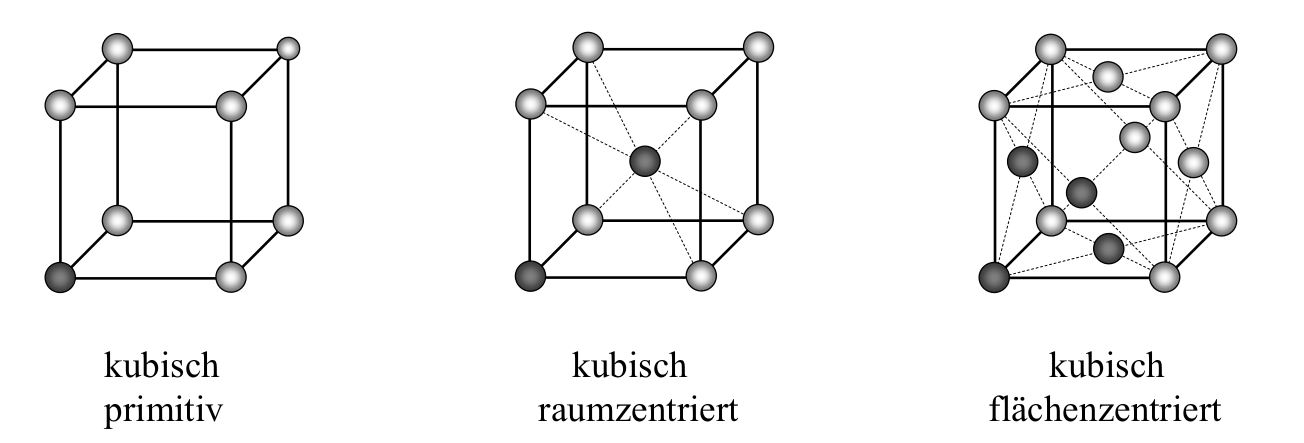
\includegraphics[width=0.9\textwidth]{Abb/kubische_gitter.png}
    \caption{Die drei kubischen Atomgitter. Von links nach rechts: 
             einfach kubisch (sc), kubisch raumzentriert (bcc),
             kubisch flächenzentriert (fcc)}
    \label{kub}
    % Hunklinger
\end{figure}
Es existieren drei verschiedene kubische Gitter.
Diese sind in Abbildung \ref{kub} dargestellt. Im Rahmen dieses Versuches
soll nur das kubisch flächenzentrierte Gitter näher betrachtet werden. Viele Metalle
und Legierungen kristallisieren in diese Anordnung.\\
\begin{figure}
    \centering
    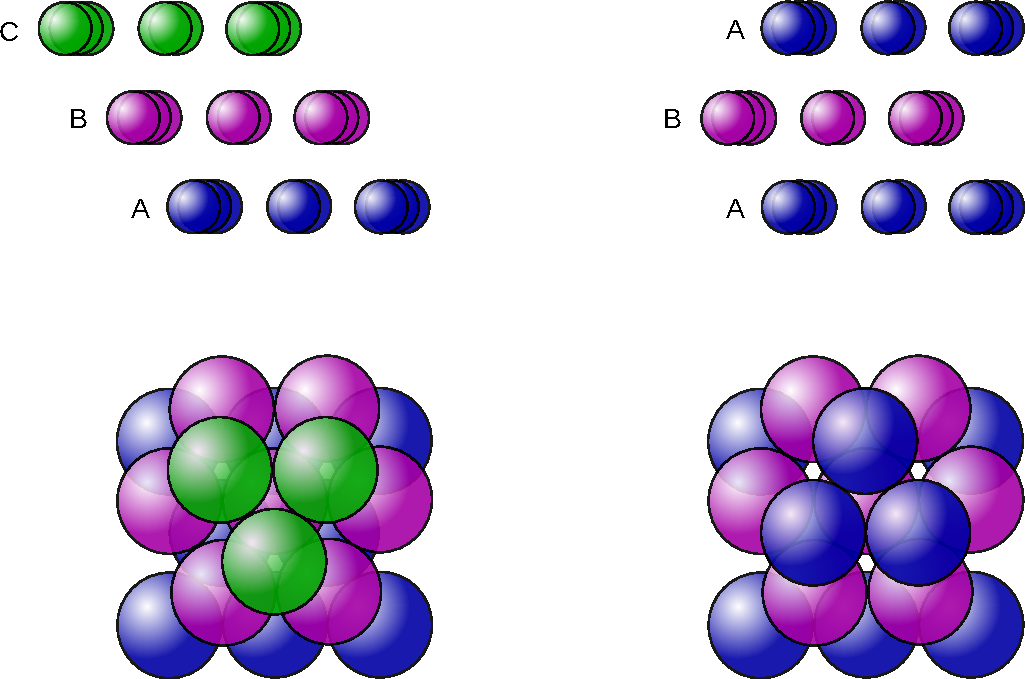
\includegraphics[width=0.7\textwidth]{Abb/DichtesteKugelpackung.pdf}
    \caption{Die möglichen Stapelfolgen für eine dichteste Kugelpackung:
             Links im Bild werden drei verschiedene Schichten gestapelt,
             also ABCABC... 
             Rechts werden nur zwei Schichten gestapelt, die dritte Schicht liegt
             also exakt auf der Ersten, ABABAB...}
    \label{pack}
    % https://de.wikipedia.org/wiki/Dichteste_Kugelpackung
\end{figure}
Betrachtet man eine möglichst dichte Packung an Kugeln, so sind zwei Stapelfolgen 
möglich. Das fcc-Gitter repräsentiert hierbei die Schichtfolge ABCABC..., siehe 
hierzu Abbildung \ref{pack}. Ein Atom hat in dieser Anordnung 12 nächste Nachbarn
mit dem Abstand $\frac{a}{\sqrt{2}}$. $a$ sei hier die Gitterkonstante des Würfels.
In einer kubischer Zelle befinden sich $8 \cdot \frac{1}{8} + 6 \cdot \frac{1}{2} 
= 4$ Atome. Die Atome an den Ecken befinden sich in acht Zellen gleichzeitig, jene 
an den Flächen in zwei. Sie werden deshalb anteilig hinzugerechnet.
Die Packungsdichte $ V_{\text{Atome}} / V_{\text{kub. Zelle}} $ ergibt sich somit zu:
\[
    \underset{\text{Volumen eines Atoms}}{
        \underbrace{
            \frac{4}{3} \left( \frac{d_{NN}}{2} \right)^2 \pi}} \cdot
    \underset{\text{Atome pro kubischer Zelle}}{4} 
    / \, 
    \underset{\text{Volumen des Würfels}}{a^3} \approx 0.74
\]
Die dichtest mögliche Kugelpackung nimmt also $74\%$ des Raums ein.
% Hunklinger
\newpage

        \subsubsection{Hexagonal dichteste Kugelpackung}

\begin{wrapfigure}{r}{0.45\textwidth}
    \centering
    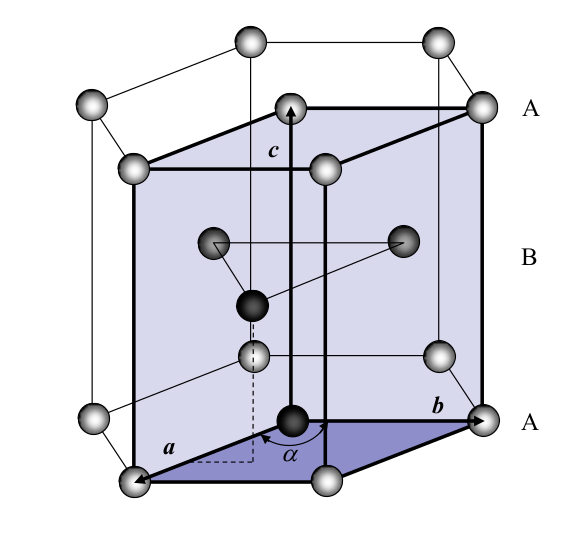
\includegraphics[width=0.4\textwidth]{Abb/hcp.png}
    \caption{hcp-Gitter}
    \label{hcp}
    % Hunklinger
\end{wrapfigure}
Die rechte Stapelfolge in Abbildung \ref{pack} wird als hexagonal dichteste
Kugelpackung (hcp) bezeichnet. In Eigenschaften wie Abstand und Anzahl der nächsten
Nachbarn gleicht es dem fcc, was durch die Betrachtung als dichteste Packungen 
schnell klar wird. In Abbildung \ref{hcp} sind die Stapelfolgen eingezeichnet.
Die Vektoren $a$ und $b$ sind gleich lang. Für $c$ findet man $c = \sqrt{ 
\frac{8}{3}} \, a$. In realen Kristallen weicht dies oft etwas ab.
% Hunklinger

        \subsubsection{Graphenstruktur}

\begin{figure}
    \centering
    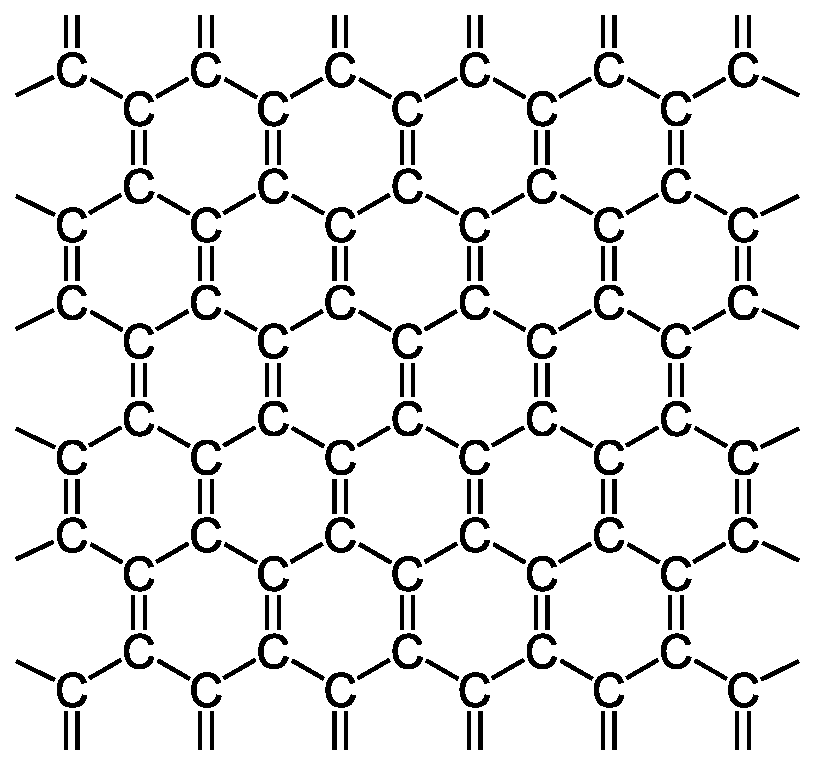
\includegraphics[width=0.4\textwidth]{Abb/graphenstruktur.pdf}
    \caption{Struktur von Graphen}
    \label{graphenstruktur}
    % https://de.wikipedia.org/wiki/Graphen
\end{figure}
In Abbildung \ref{graphenstruktur} ist die Bienenwabenstruktur des Graphens 
dargestellt. Es handelt sich um eine Atomlage von Kohlenstoffatomen, die durch
sp2-Hybridorbitale verbunden sind. Alle Bindungen sind hierbei gleich lang.
% Hunklinger

    \subsection{Quantenmechanisches Tunneln}
    \subsection{Piezoelektrischer Effekt}

\section{Aufbau eines Rastertunnelmikroskops}
    \subsection{Aufbau der Spitze}
    \subsection{Herstellung der Spitze}
    \subsection{Piezomotoren}

\section{Betriebsarten eines Rastertunnelmikroskops}
    \subsection{Topographischer Modus}
    \subsection{Modus konstanter Höhe}
    \subsection{Spektroskopie}

\section{Probenmaterialien}
    \subsection{Graphit}
    \subsection{Gold}
    \subsection{Molybdänsulfit}
